


\begin{figure}[tbp]
\centering


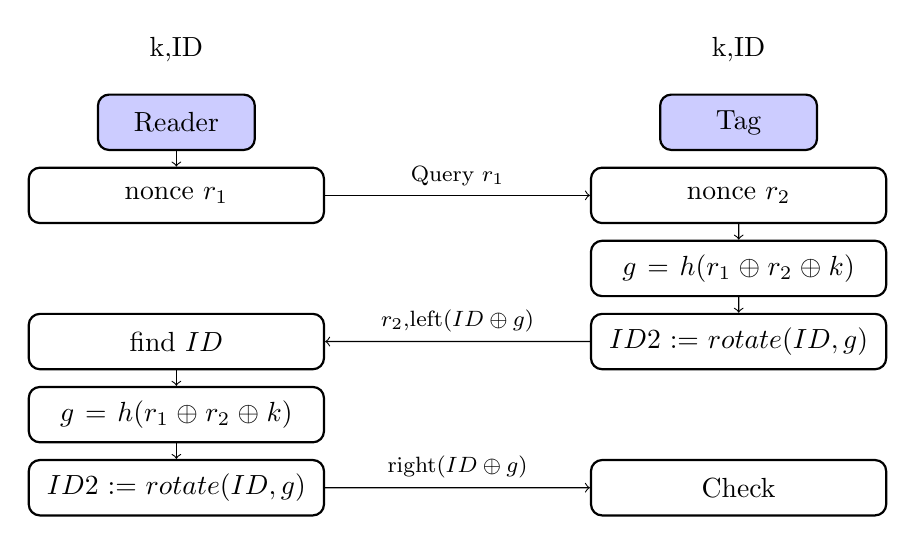
\begin{tikzpicture}[yscale=-0.91,scale=1.02,
 block/.style ={rectangle, draw=black, thick, fill=white, text width=10em,align=center, rounded corners, minimum height=2em},
 block1/.style ={rectangle, draw=black, thick, fill=blue!20, text width=5em,align=center, rounded corners, minimum height=2em},
 line/.style ={draw, thick, -latex',shorten >=2pt},
 cloud/.style ={draw=red, thick, ellipse,fill=red!20,
 minimum height=1em}]

\draw (0,1) node[block1] (Rtop) {Reader};
\draw (0,0) node[] (upper1) {k,ID};
\draw (7,1) node[block1] (Ttop) {Tag};
\draw (7,0) node[] (upper2) {k,ID};


\draw (0,2) node[block] (R1) {nonce $r_1$};

\draw (7,2) node[block] (T1) {nonce $r_2$};
\draw (7,3) node[block] (T2) {$g=h(r_1\oplus r_2 \oplus k)$};
\draw (7,4) node[block] (T3) {$ID2 := rotate(ID,g)$};

\draw (0,4) node[block] (R2) {find $ID$};
\draw (0,5) node[block] (R3) {$g=h(r_1\oplus r_2 \oplus k)$};
\draw (0,6) node[block] (R4) {$ID2 := rotate(ID,g)$};

\draw (7,6) node[block] (T4) {Check};

%	\node [fill=white, draw=black, shape=circle, minimum size=8mm] (1) at (0, 0) {1};
%	\node [fill=white, draw=black, shape=circle, minimum size=8mm] (2) at (1, 0) {2};
%	\node [fill=white, draw=black, shape=circle, minimum size=8mm] (4) at (2, 0) {4};
%	\node [fill=white, draw=black, shape=circle, minimum size=8mm] (7) at (3, 0) {7};

	\draw [fill=none, ->] (Rtop) to (R1);
	\draw [fill=none, ->] (R1) to node[above,pos=0.5]{\footnotesize Query $r_1$} (T1);
	\draw [fill=none, ->] (T1) to (T2);
	\draw [fill=none, ->] (T2) to (T3);
	
	\draw [fill=none, ->] (T3) to node[above,pos=0.5]{\footnotesize $r_2$,left($ID\oplus g$)} (R2);
	\draw [fill=none, ->] (R2) to (R3);
	\draw [fill=none, ->] (R3) to (R4);
	\draw [fill=none, ->] (R4) to node[above,pos=0.5]{\footnotesize right($ID\oplus g$)} (T4);
	

\end{tikzpicture}

\caption{Flow of procesing of the CH07 verification protocol}\label{fig:pentominos_subfigure}
\end{figure}





